\section{Linear Propagation in Two-level Atoms}
  \label{sec:propagation_twolevel}

  % \subsection{Intro}

    Now that we have derived the necessary differential equations to describe
    \textsc{1d} propagation in an atomic vapour and described computational
    algorithms for the numerical solution of the problem for a given set of
    boundary conditions, we will look at example results from simulated
    propagation of a monochromatic (\ie single carrier frequency) field in a
    simple two-level system.

    We will define the two-level system and present the results of propagation
    for some boundary conditions representative of laboratory experiments:
    pulsed and continuous-wave (\textsc{cw}) input fields. We'll then make an
    analysis of the frequency dependent behaviour of the simulated propagation
    of a wider-spectrum field. We will use these results to verify that these
    results match the known analytic response functions for the linear regime,
    such that we have confidence in the computational scheme for the
    simulations we will later obtain for nonlinear systems with more than one
    carrier frequency.

    We will also introduce the natural unit system which will be used throughout
    this thesis.

  \subsection{The Two-level System}

    No real atomic system exists with only two levels of course, but this
    minimal scheme is a good approximation in the case of resonant interaction
    with a well-separated transition.

    The system is defined by a Hilbert space covered by a basis that consists of
    a   ground state $\Ket{0}$ and an excited state $\Ket{1}$ with eigenenergies
    $E_0$ and $E_1$. The resonance frequency $\omega_0 = (E_1 - E_0)/\hbar$. As
    is conventional we define the detuning of the input carrier frequency from
    resonance as $\Delta = \omega - \omega_0$ and the complex Rabi
    frequency\cite{loudon2000quantum}
    \begin{equation}
      \Omega(z,t) =
      \frac{d_{01}}{\hbar} \mathcal{E}(z,t)
    \end{equation}
    where $d_{01} = \Bra{0} \mathrm{d} \Ket{1}$ is the transition dipole matrix element.

    The time evolution is independent of the absolute value of the bare state
    energies, so we may set the ground state energy $E_0 = 0$. Making the
    rotating wave approximation, we find that the atomic Hamiltonian is given by
    \begin{equation}
      \mathcal{H} = \hbar
      \begin{bmatrix}
        0 & \nicefrac{\Omega}{2} \\
        \nicefrac{\Omega^*}{2} & -\Delta
      \end{bmatrix}
    \end{equation}
    in the frame rotating with the carrier frequency.\cite{allen1975optical}

    For the Lindblad superoperator $\mathcal{L}$ we have just a single collapse
    operator representing spontaneous decay of the electron from the the excited
    state to the ground state
    \begin{equation}
      C = \sqrt{\Gamma}\Ket{0}\!\Bra{1}.
    \end{equation}

    In two-level medium we only have one dipole matrix element and one coherence
    to consider, such that (neglecting the Doppler effect for now) the
    propagation equation (\ref{eqn:comoving_mwe}) may be written
    \begin{equation}
      \frac{\partial}{\partial z}\mathcal{E}(z,t') = 
          \ii N(z) \frac{k}{2 \varepsilon_0} d_{01} \cdot \rho_{01}(z,t').
      \label{eqn:twolevel_field_eqn}
    \end{equation}
    It is useful to write the propagation now in terms of the Rabi frequency
    \begin{equation}
      \frac{\partial}{\partial z}\Omega(z,t') = \ii N(z) g \cdot \rho_{01}(z,t')
    \end{equation}
    where we define a propagation coefficient
    \begin{equation}
      g_{01} = \frac{d_{01}^2 k}{2 \varepsilon_0 \hbar}
    \end{equation}
    which is constant for a given transition with dipole matrix element $d_{01}$
    and for a field with carrier wavenumber $k$.

  \subsection{The Natural Unit System}

    For a two-level system we have a single natural linewidth, and so it is
    convenient to introduce a natural unit system, with frequencies in units of
    the natural linewidth $\Gamma$, times in terms of the reciprocal spontaneous
    decay lifetime $\tau = 1/\Gamma$ and distances in terms of the length of the
    medium $L$.

    To give an illustrative example, we will take a rubidium 85 cell and apply a
    monochromatic field on resonance with the \textsc{d1} transition from the
    $5^2\mathrm{S}_{\nicefrac{1}{2}}$ ground state to the
    $5^2\mathrm{P}_{\nicefrac{1}{2}}$ excited state at $\omega =
    \unit[2\pi\times377]{THz}$. The spontaneous decay rate for the transition
    $\Gamma = \unit[2\pi\times5.75]{MHz}$ such that the lifetime $\tau =
    \unit[27.6]{ns}$. The transition dipole matrix element is $d_{01} =
    \unit[2.53\cdot10^{-29}]{C~m}$. From this we can calculate that the
    propagation coefficient for the transition $g_{01} =
    \unit[2\pi\times4.34\cdot10^{-9}]{MHz~cm^2}$.

    The number density $N$ in a contained cell is a function of the temperature
    of the cell. For an example temperature $T = \unit[200]{\textdegree C}$ we
    have $N = \unit[9.26\cdot10^{14}]{cm^{-3}}$. If we then take a cell of a
    typical length $L = \unit[1]{mm}$, the key parameter we require for
    describing propagation in the medium can be expressed purely in terms of the
    natural units as $N g_{01} = \unit[2\pi\times70]{\Gamma /L}$.

    By introducing this natural unit system we are able to reduce the number of
    parameters involved in the mathematical problem. For example, it becomes
    clear that increasing the length of the medium ten times is equivalent to
    raising the number density by the same scale, or by choosing a system with a
    suitably higher dipole moment.

  \subsection{Weak Probe Lineshape}    

    The Lindblad master equation (\ref{eqn:lindblad}) represents a set of
    differential equations in time for the time evolution of each density matrix
    element.

    As we know via equation (\ref{eqn:polarisation_coherences}) that the
    polarisation $\mathcal{P}$ is related to the off-diagonal coherence
    $\rho_{01}$, we write out the particular equation to follow its time
    evolution, such that
    \begin{equation}
      \label{eqn:twolevel_coh_master_eqn}
      \frac{\dd \rho}{\dd t} = \ii \Omega \left( \rho_{00} - \rho_{11} \right) + \left( \ii \Delta - \frac{\Gamma}{2} \right) \rho_{10}.
    \end{equation}

    In the case of weak field input on the medium, we may assume that we're in a
    quasi-static regime where the atomic density matrix changes negligibly over
    the time of the input. We thus set the time derivative in equation
    (\ref{eqn:twolevel_coh_master_eqn}) to zero.

    The initial condition is that all of the atomic population starts in the
    ground state. For a weak field we may also assume that population transfer
    is negligible such that $\rho_{11} = 0$.

    Under these weak field approximations, we may thus derive the steady state,
    weak field lineshape
    \begin{equation}\label{eqn:weak_lineshape}
      \rho_{01}(z) = -\Omega(z) \frac{1}{\ii \frac{\Gamma}{2} + \Delta}.
    \end{equation}

  \subsection{Weak Pulse Propagation Results}    

    The first Maxwell-Bloch simulation results we will consider are for an input
    field profile of finite duration, namely a Gaussian pulse. In general for
    short duration pulses, the atoms do not reach equilibrium with the applied
    field before the pulse has passed, however for weak fields so little
    population is transferred that a quasi-static regime can be a good
    approximation. In the following simulations we solve the full Maxwell-Bloch
    problem in order to compare to the analytically known equation
    (\ref{eqn:twolevel_coh_master_eqn}).

    The Gaussian pulsed input field is defined by
    \begin{equation}
      \Omega(t) = \Omega_{0} \exp \left[ -4 \log 2 \left( \frac{t - t_0}{t_w}
                              \right)^2 \right]
      \label{eqn:gaussian}
    \end{equation}
    where $\Omega_{0}$ is the peak input Rabi frequency, $t_0$ is the time at
    which the function reaches that peak, and $t_w$ is the full width at half
    maximum (\textsc{fwhm}) of the pulse.

    In this simulation we let the peak $\Omega_0 =
    \unit[2\pi\times10^{-3}]{\Gamma}$, the centre $t_0 = 0$ and the width $t_w
    =$~\unit[$0.1$]{$\tau$}. We define the medium to have a length $L$, number
    density $N$ and coupling $g$ such that the key absorption parameter $Ng =
    \unit[2\pi\times1]{\Gamma /L}$.

    \begin{figure}
      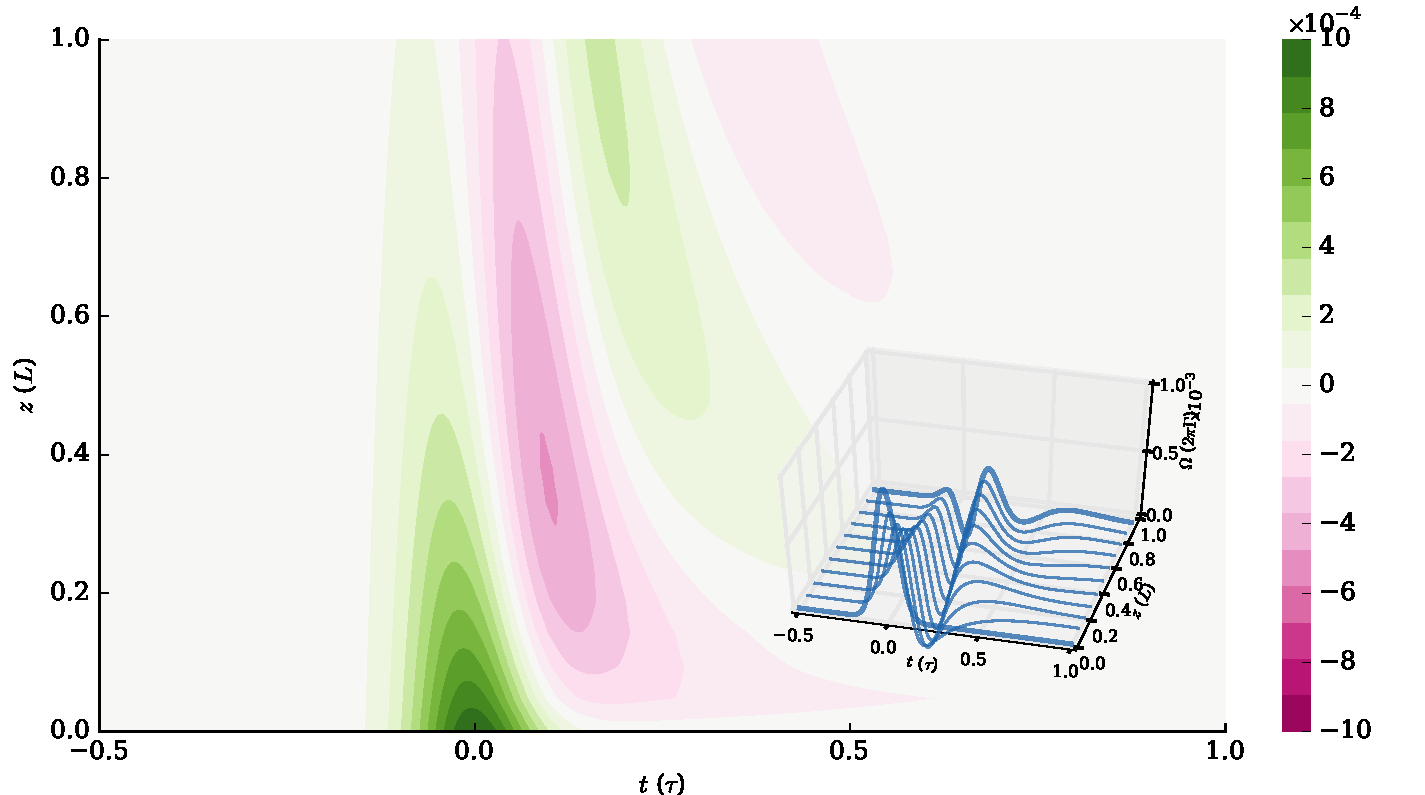
\includegraphics[width=\linewidth]{figs/02_propagation/mb_two_solve_wp_t01_Ng0100_T0_vel0_D0_fig1.pdf}
      \caption{
      The real part of the complex Rabi frequency $\Omega(z,t)$ showing the
      simulated result of propagation of a weak pulse through a two-level
      medium. (Inset \textsc{3d}) The field has Gaussian profile entering the
      medium at $z=0$, with peak $\Omega_0 = \unit[2\pi\times10^{-3}]{\Gamma}$
      and width $t_w =$~\unit[$0.1$]{$\tau$}.
      }
      \label{fig:pulse_field}
    \end{figure}

    In figure \ref{fig:pulse_field} we present a colour map of the simulated
    real part of the complex Rabi frequency $\Omega(z,t)$ describing the field
    profile as it propagates through the medium.

    Time $t$ is shown on the $x$-axis and the propagation distance $z$ is shown
    on the $y$-axis such that the field enters at the bottom of the plot. The
    horizontal slice at $z = 0$ thus represents the Gaussian input field. All
    propagation results are presented in the speed-of-light reference frame
    described in section \ref{sec:propagation_ali}.

    We see that the primary pulse envelope is attenuated and slightly fast, such
    that the first peak arrives at the rear of the medium, $z = \unit[1]{L}$, at
    a time $t \approx $\unit[$-0.05$]{$\tau$} in the speed-of-light reference
    frame. [normal dispersion profile]. Not all of the energy of the pulse is
    absorbed, however. This is because the pulse is short in duration relative
    to $\tau$, such that its spectral profile is wider in frequency space than
    the absorption window of the atoms. Thus some spectral components of the
    field see a medium which is transparent to them. However, they remain
    subject to phase shift. We see high-frequency ringing, also described as a
    $0\pi$ pulse as the total area integrates to zero.\cite{allen1975optical, Durrant1976}

    \begin{figure}
    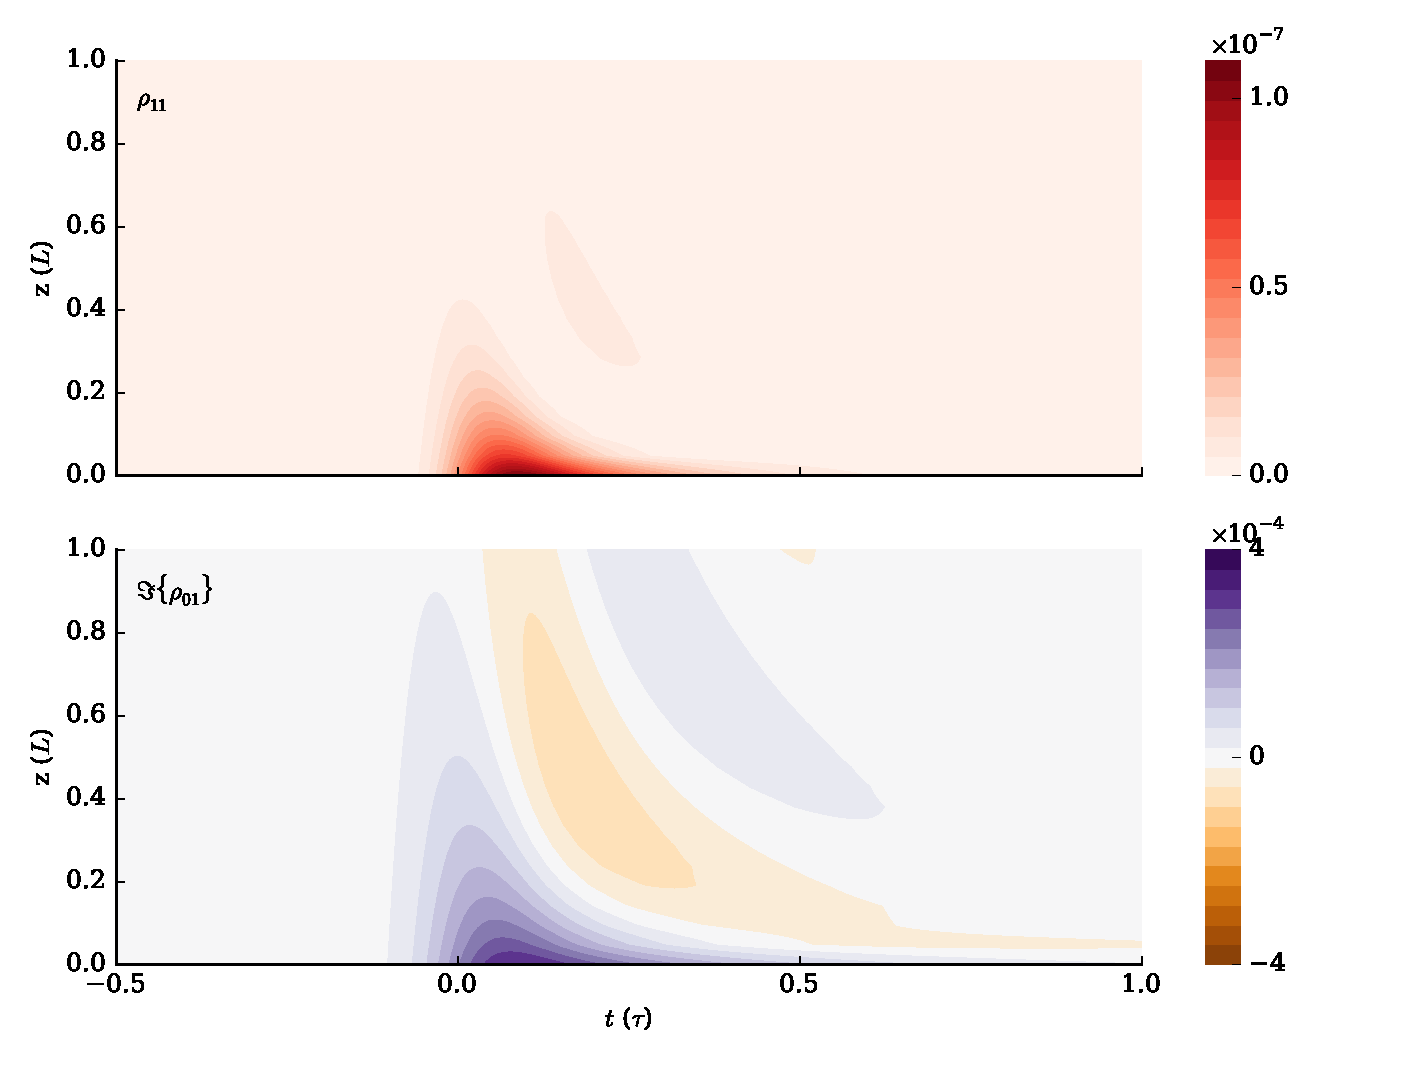
\includegraphics[width=\linewidth]{figs/02_propagation/mb_two_solve_wp_t01_Ng0100_T0_vel0_D0_fig2.pdf}
    \caption{
      Density matrix elements of the two-level atom system as a function of $z$
      and $t$ during the simulation. (Top) Excited state population
      $\rho_{11}(z,t)$. (Bottom) Coherence $\rho_{01}(z,t)$ between the states.
      The simulation parameters and boundary conditions are as for figure
      \ref{fig:pulse_field}.
    }
    \label{fig:pulse_pop_coh}
    \end{figure}

    In figure \ref{fig:pulse_pop_coh} we present colour maps of simulated
    density matrix elements describing the response of the atoms along the
    medium as the applied field reaches them.

    The cumulative Rabi frequency of the pulse is many orders of magnitude too
    small to saturate the excited state population so that for the atoms at the
    front of the medium at $z\!=\!0$, $\rho_{11}$ continues to rise through the
    pulse to a peak at time $t \approx~$\unit[$0.01$]{$\tau$} after the input
    field has peaked. There is a small `echo' in the excited state, due to the
    field ringing, visible at $t \approx~$\unit[$0.2$]{$\tau$} and between $z =
    \unit[0.4]{L}$ and $\unit[0.6]{L}$.

    A positive imaginary coherence $\Im[{\rho_{01}}]$ is driven by the applied
    field at the front of the medium. We observe that the coherence decays at
    half the rate of the excited state population, $\nicefrac{\Gamma}{2}$,
    consistent with equation (\ref{eqn:twolevel_coh_master_eqn}).

  \subsection{Spectral Analysis}

    In section \ref{sec:propagation_susc} we made use of Fourier transforms to
    shift perspective to the frequency domain. We showed that in the linear
    regime it is possible to derive a response function, given in equation
    (\ref{eqn:lin_pol_freq}), which when substituted into the propagation
    equation allows us to understand how the susceptibility describes the
    frequency-dependent absorptive and dispersive properties of a medium with
    respect to a weak field.

    In order to verify the numerical model we have developed, as well as to
    demonstrate these spectral properties, we will now look at results from a
    simulation of a pulse propagating through the two-level medium. We wish to
    confirm that the results of the simulation match the known analytic response
    functions for the linear regime.

    \begin{figure}
    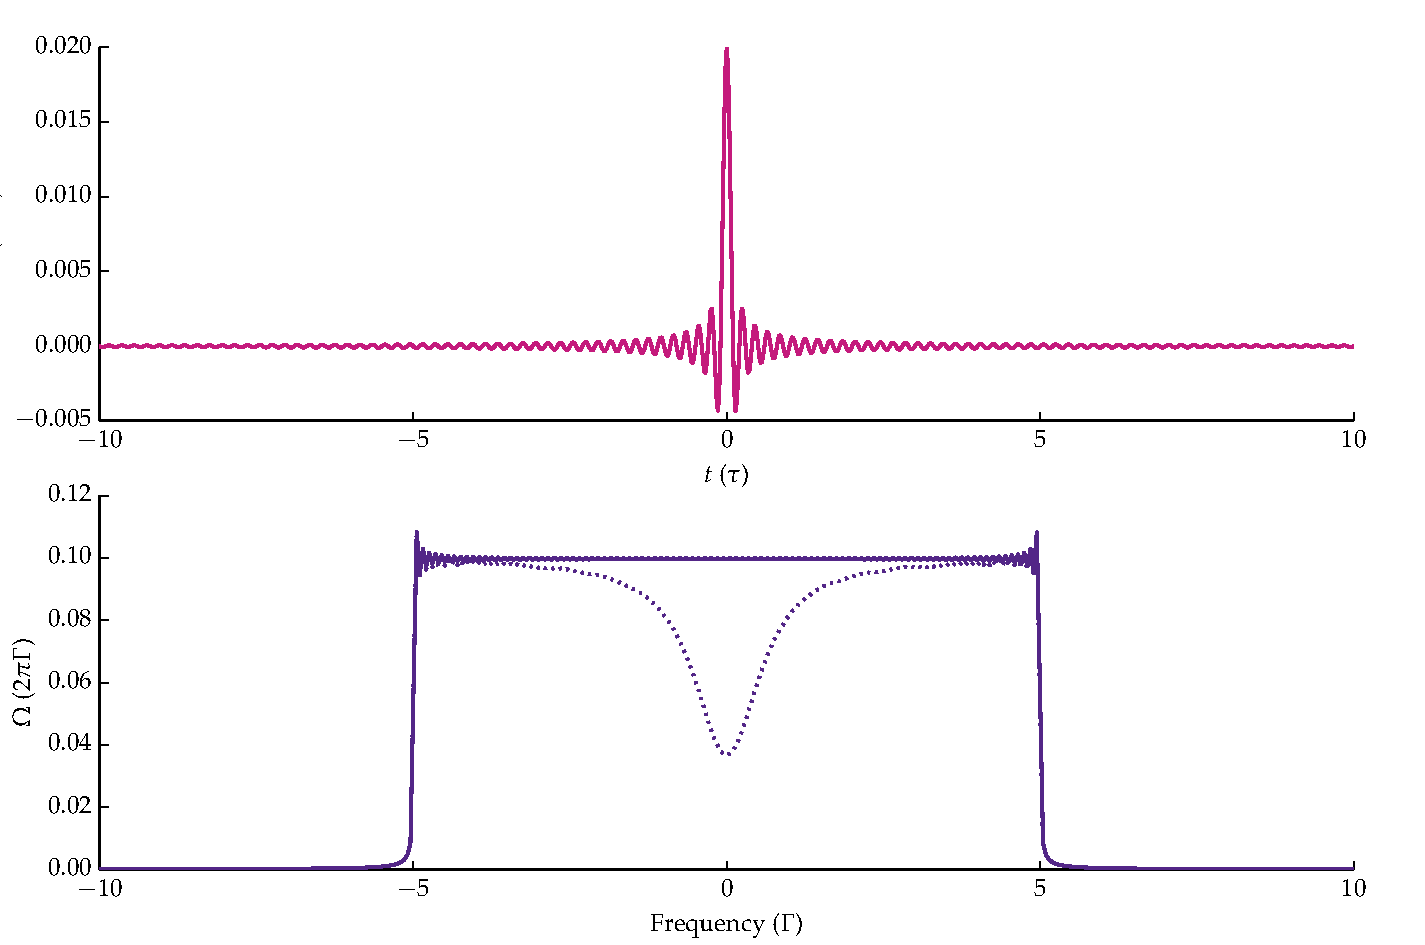
\includegraphics[width=\linewidth]
      {figs/02_propagation/two_mb_solve_f03_fig2.pdf}
    \caption{
    (Top) The sinc function (pink) defined by equation (\ref{eqn:sinc}) which
    forms a simulated pulse profile in time $\Omega(t,0)$ entering the medium at
    $z=0$, \ie the boundary condition. (Bottom) (Purple solid) The discrete
    Fourier transform $\lvert \Omega(\omega,0) \rvert$ of the sinc shape above,
    representing the same function in the frequency domain at $z=0$. (Purple
    dotted) The resulting field profile $\lvert \Omega(\omega,z=1) \rvert$ in
    the frequency domain at $z = \unit[1]{L}$, after propagation through the
    medium. The medium is defined with a length $L$, number density $N$ and
    coupling $g$ such that $Ng = \unit[2\pi~1]{\Gamma /L}$.
    }
    \label{fig:sinc_time_freq}
    \end{figure}

    For this simulation we define an unusual and artificial time profile for the input field boundary condition: a cardinal sine (sinc) function given by
    \begin{equation}\label{eqn:sinc}
      \Omega(t) = \frac{1}{20 \sqrt{2 \pi}} \mathrm{sinc}(10 t).
    \end{equation}

    This input profile, shown in the top subplot of figure
    \ref{fig:sinc_time_freq}, is clearly impractical for any experimental setup.
    We choose this profile because its Fourier transform, shown in the bottom
    subplot of figure \ref{fig:sinc_time_freq}, is a square function with a
    width of $\unit[10]{\Gamma}$. This gives us a wide spectral range over which to observe the effect of the two-level medium on the field.

    The discrete Fourier transform (\textsc{dft}) is used as the numerical
    method for shifting to the frequency domain, which results in some Gibbs
    ringing\cite{Hewitt1979} seen at the corners at $\unit[\pm 5]{\Gamma}$.

    A more-realistic Gaussian time profile, short in duration, would also cover
    a wide spectral range. We choose the sinc function for the reason that it
    provides greater accuracy in the wings far away from resonance, where both
    the input and output field amplitudes would be extremely small for the
    Gaussian function, bringing inaccuracy as we get close to limits for
    floating point storage.

    The absorptive effect of the medium is immediately visible if we compare the
    $\lvert \Omega(\omega, z\!=\!1) \rvert$, the profile at the back of the
    medium, also shown (dotted) in the bottom subplot of figure
    \ref{fig:sinc_time_freq}. Around resonance there is a significant dip of
    around $60\%$ in the transmitted Rabi frequency (and thus the electric field
    amplitude).

    \begin{figure}[]
    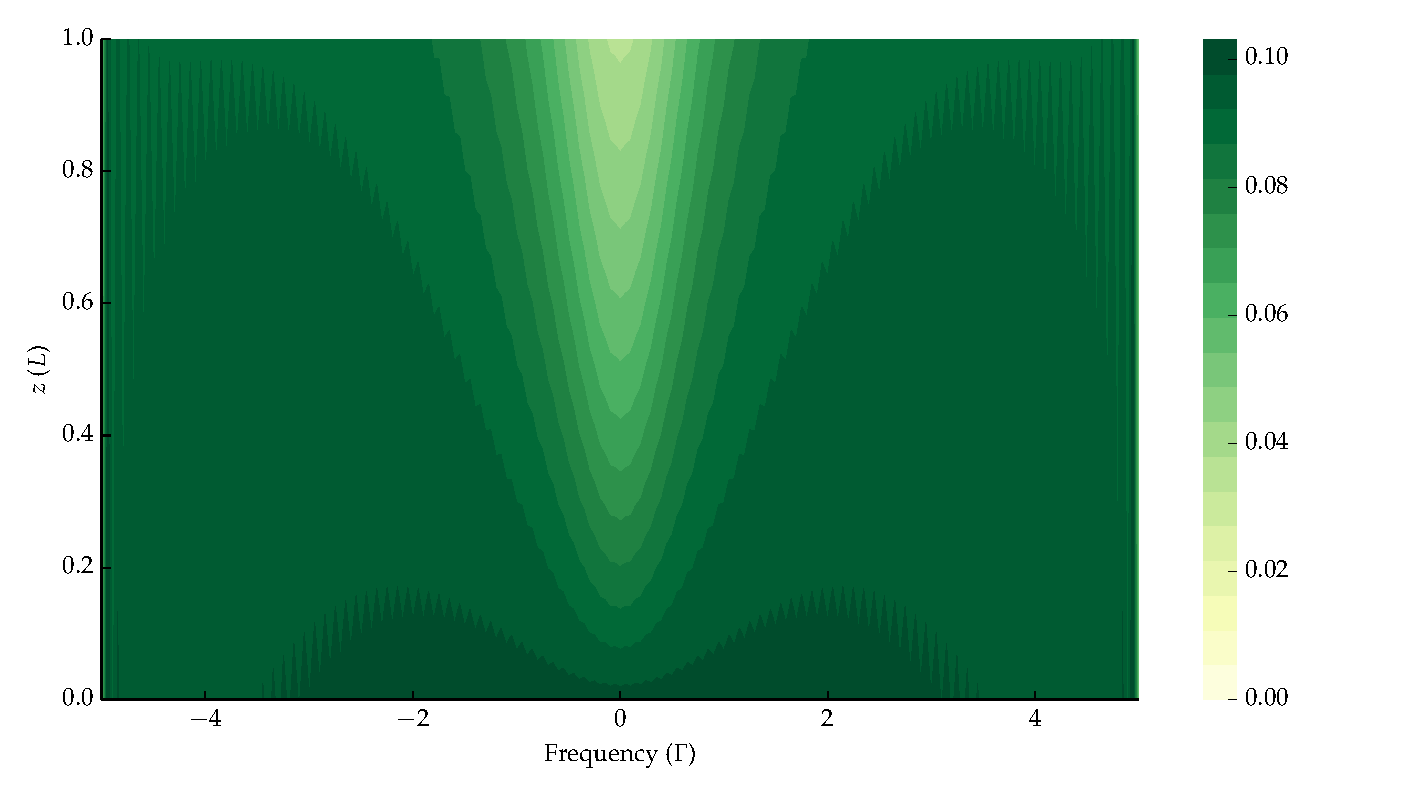
\includegraphics[width=\linewidth]
      {figs/02_propagation/two_mb_solve_f03_fig1.pdf}
    \caption{
    Magnitude of the Fourier-transformed Rabi frequency $\lvert \Omega(z,\omega)
    \rvert$, showing propagation of the field through the medium in the
    frequency domain during the simulation. The input boundary condition field
    profile at $z=0$ is the sinc function shown in figure
    \ref{fig:sinc_time_freq}. The medium is defined with a length $L$ and number
    density $N$ such that  $Ng = \unit[2\pi~1]{\Gamma /L}$.
    }
    \label{fig:sinc_freq_zt}
    \end{figure}

    In figure \ref{fig:sinc_freq_zt} we show the results for $\lvert
    \Omega(\omega, z) \rvert$ as the sinc pulse moves through the medium. On resonance, the field decays exponentially while in the spectral wings we see nearly full transmission.

    We can compare the simulated result with the analytic expression given in
    equation  (\ref{eqn:efield_susc_real_imag}), which tells us that we can
    obtain  the imaginary part of the susceptibility by checking the attenuation
    of the field via
    \begin{equation}\label{eqn:chi_im_sim}
      \frac{k}{2} \chi_I(\omega) z = -\log{\frac{\lvert \Omega(z, \omega) \rvert}{\lvert \Omega(z=0, \omega) \rvert}}
    \end{equation}
    and the real part of the susceptibility by checking the phase shift over the medium,
    \begin{equation}\label{eqn:chi_re_sim}
      \frac{k}{2} \chi_I(\omega) z = \phi(z, \omega) - \phi(z=0, \omega)
    \end{equation}
    where the $\phi$ is defined via
    \begin{equation}
      \Omega(z, \omega) = \lvert \Omega \rvert \ee^{i \phi}.
    \end{equation}

    \begin{figure}[]
    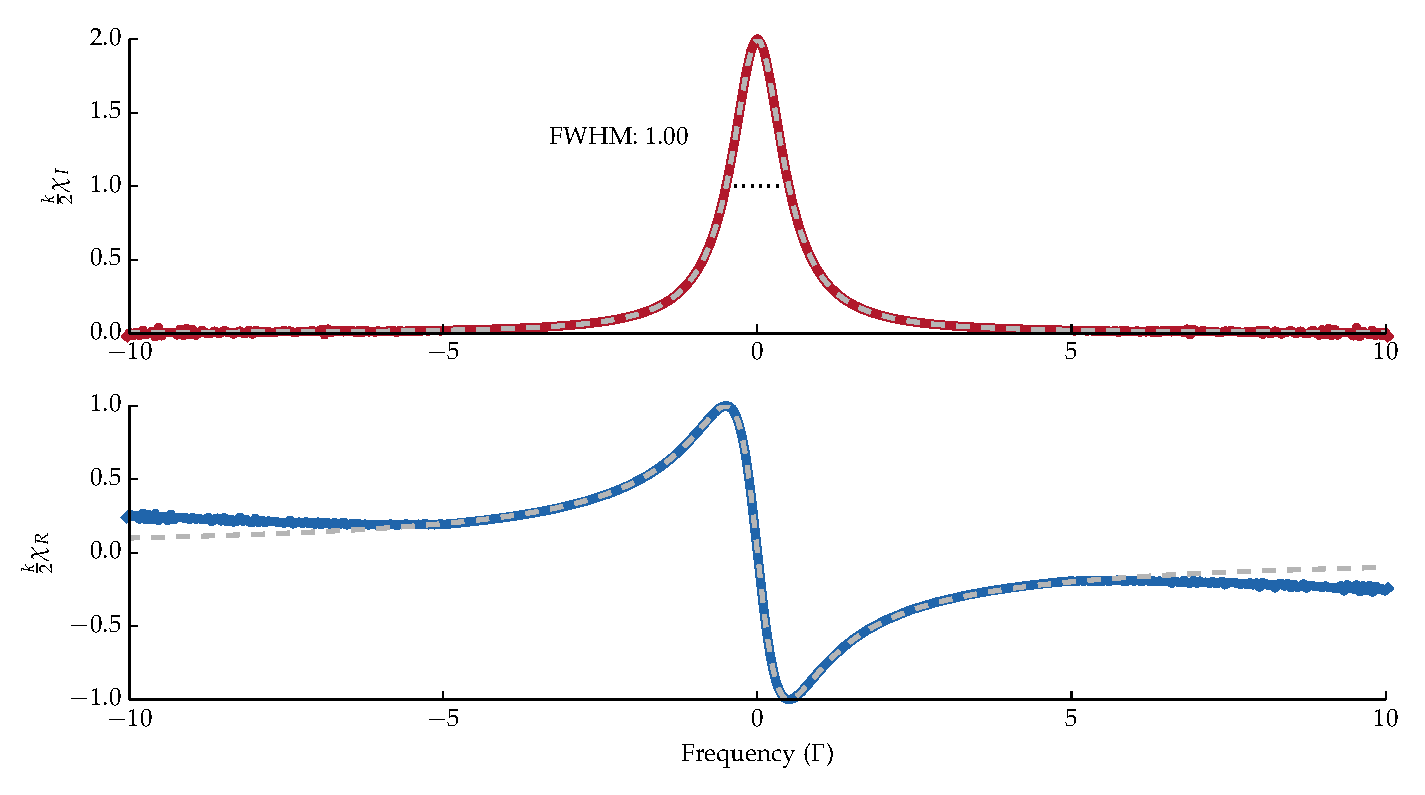
\includegraphics[width=\linewidth]
      {figs/02_propagation/two_mb_solve_f03_fig5.pdf}
    \caption{
    (Top) (red solid) The imaginary part of the linear susceptibility $\chi_I$
    derived from the simulation via equation (\ref{eqn:chi_im_sim}). (Bottom)
    (blue solid) The real part of the linear susceptibility $\chi_R$ derived from
    the simulation via equation (\ref{eqn:chi_re_sim}). (grey dashed) Analytic
    functions of $\chi_I$ and $\chi_R$ derived from the weak probe lineshape given
    in equation (\ref{eqn:chi_weak_probe}). The \textsc{fwhm} of the $\chi_I$
    lineshape is shown as measured numerically.
    }
    \label{fig:susc_imag_real_linear_comp}
    \end{figure}

    In figure \ref{fig:susc_imag_real_linear_comp} we present the simulated
    results for the susceptibility as defined in (\ref{eqn:chi_im_sim}) and
    (\ref{eqn:chi_re_sim}).

    We see that the imaginary part, describing absorption of the field, has the
    Lorentzian lineshape familiar as a solution for classical systems involving
    forced and damped resonance. The \textsc{fwhm} is measured numerically, and
    as we would expect it is equal to $\unit[1]{\Gamma}$, the natural linewidth
    around which we designed the natural unit system.

    Absorption linewidths observed in experiment will in general be
    significantly wider, as the important effects of Doppler broadening and
    atomic collisions must be considered. This natural linewidth represents the
    theoretical minimum linewidth that could be observed for cold atoms due to
    spontanous emission rate, which for an atom in free space can never be
    reduced.\cite{loudon2000quantum}

    The real component has the familiar dispersion lineshape describing the
    phase of the input field relative to the frequency of the oscillator as it
    passes over resonance from lagging to leading\cite{hecht2015optics}.

    By comparing the linear propagation equation (\ref{eqn:fo_mwe_linear})
    with the weak probe approximation for the coherence, given in equation
    (\ref{eqn:weak_lineshape}), we note that we can also derive an analytic
    expression for the frequency-dependent susceptibility in this regime,
    \begin{equation}\label{eqn:chi_weak_probe}
        \frac{k}{2} \chi(\omega) = -Ng \frac{1}{\ii \frac{\Gamma}{2} + \Delta}.
    \end{equation}

    The real and imaginary parts of this function are overlaid (grey dashed
    lines) on the simulated results and we see excellent agreement around
    resonance. We see in (\ref{eqn:chi_weak_probe}) that the imaginary part of
    the susceptibility, and thus the absorption, is solely due to the
    spontaneous decay term $\Gamma$. This we can understand as it is this
    scattering of energy by the atoms to the environment which results in a loss
    of energy in the system.

    Spectral field components beyond $\unit[\pm 5]{\Gamma}$ are negligible (as
    defined by the sinc function, see figure \ref{fig:sinc_time_freq}) and so we
    see some noise in the result beyond this point. We also see deviation
    between the analytic and simulated results in the dispersion profile far
    from resonance, which is due to the linear susceptibility approximation
    being valid only for near-resonant components of the field.

    This result tells us that the computational scheme designed to
    model propagation of light in atomic media is accurate in the linear regime,
    which gives us confidence in the scheme for the work we will do later going beyond this weak field limit.

    \begin{figure}[]
    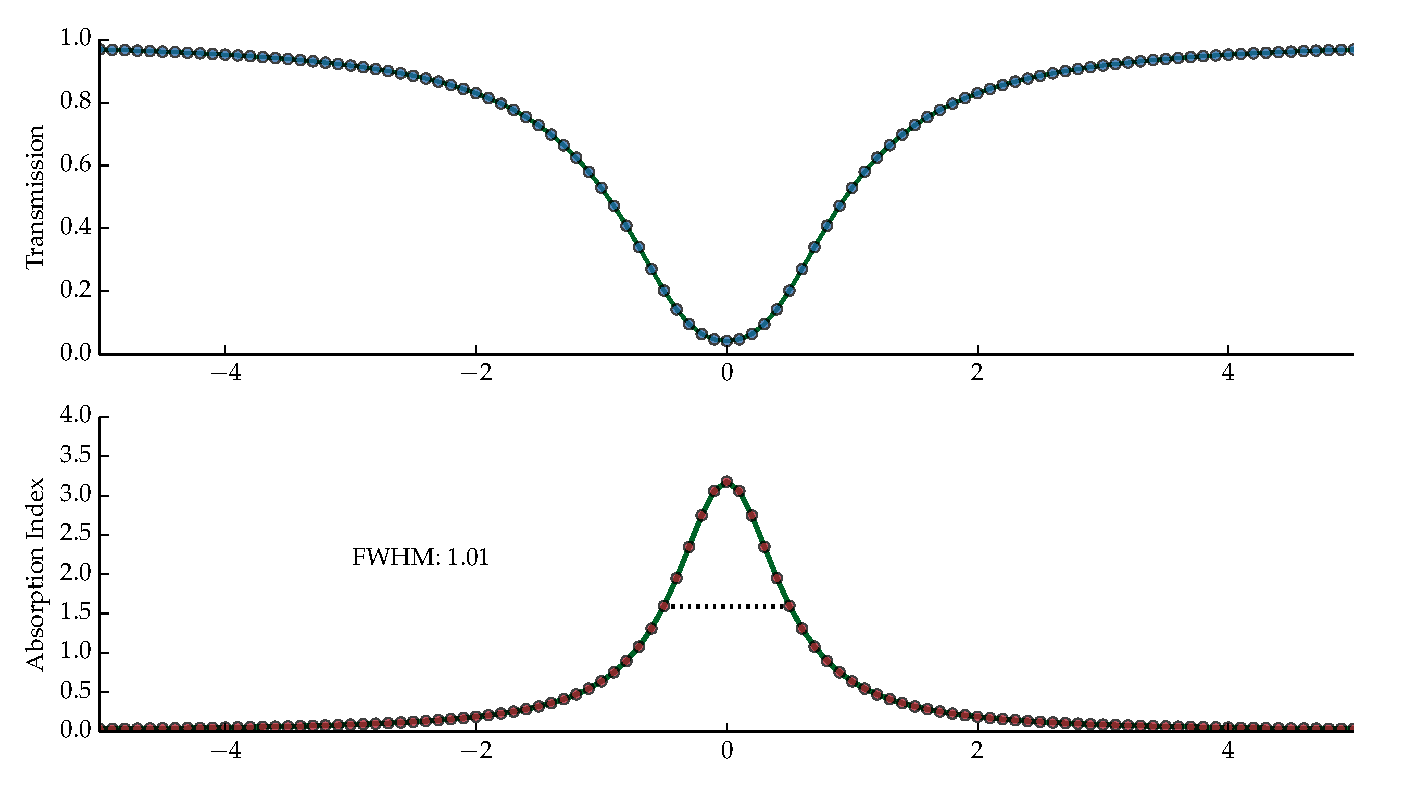
\includegraphics[width=\linewidth]{figs/02_propagation/two_mb_solve_scan_a00_fig1.pdf}
    \caption{
    Peak transmission (top) and absoptive index (bottom) for a monochromatic
    \textsc{cw} field across a discrete range of $100$ detunings $\Delta$ around
    resonance. The solid lines in both represent the same values for the
    continuous spectrum deriving from propagation of the short sinc pulse
    function.
    }
    \label{fig:linear_cw_scan_trans}
    \end{figure}

    In the scope of input field boundary conditions, at the other extreme to
    short duration, wide-spectral pulses are continuous wave (\textsc{cw})
    fields, with constant intensity over time. Such field envelopes are
    monochromatic, meaning that the frequency domain representation of a
    \textsc{cw} field in the time domain is a Dirac delta function.

    In figure \ref{fig:linear_cw_scan_trans} we make a scan of the field
    detuning $\Delta$ across resonance with the two-level atom, and mark the
    peak transmission ($T = I/I_0$) of the field along with the associated
    absorptive index.

    We also plot the transmission and absorption index of the transmission and
    absoprtion as a function of frequency for the wide-spectrum sinc pulse. The
    close agreement tells us that the short pulse's propagation is as if it were
    composed of many monochromatic frequency components interacting
    independently with the medium. In the linear regime, the solution is a
    superposition of individual frequencies.\cite{boyd2008nonlinear}

  \subsection{The Voigt Profile} % (fold)

    As mentioned, the lineshapes presented thus far for weak probe spectra
    neglect the thermal motion of the atoms, and so are only valid for atoms
    that are stationary, \ie close to absolute zero. 

    To account for thermal atoms, we must include the Doppler effect by means of
    the average over detunings described by the integral in equation
    \ref{eqn:polarisation_doppler}. The thermal lineshape function may then be expressed as
    \begin{equation}
      s(\Delta) = \int_{-\infty}^\infty h(\Delta - k v) \times f(\Delta) \dd v
    \end{equation}
    where the weak probe natural lineshape
    \begin{equation}
      h(\Delta) = -Ng \frac{1}{\ii \frac{\Gamma}{2} + \Delta}
    \end{equation}
    is given in equation (\ref{eqn:chi_weak_probe}) and $f(v)$ is the Maxwell-
    Boltzmann distribution over atomic velocities $v$ given in equation
    (\ref{eqn:max_boltz_2}).

    Using the convolution theorem for Fourier transforms, this integral can be computed as
    \begin{equation}
      s(\Delta) = \frac{\ii\sqrt{\pi}}{2u} \ee^{-z^2} \times \mathrm{erfc}(-\ii z)
      \label{eqn:voigt}
    \end{equation}
    where $z = \ii a/2  + b$ given $a = \Gamma/u$ and $b = \Delta/u$, and
    \textit{erfc} is the complementary error function.\cite{Siddons2008} This
    convolution of a Lorentzian function with a Gaussian function is known as a
    Voigt profile.

    \begin{figure}[]
      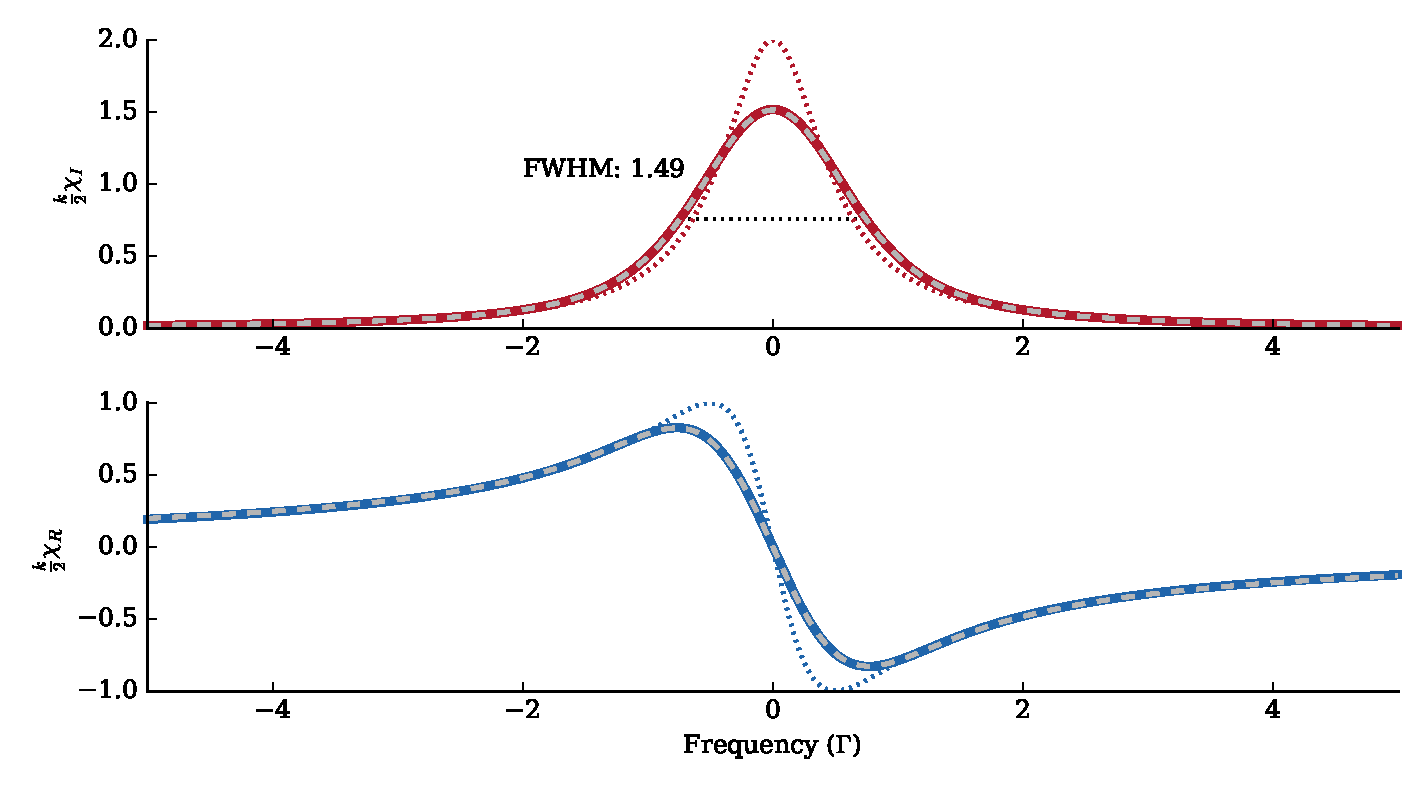
\includegraphics[width=\linewidth]{figs/02_propagation/mb_two_solve_wpdopp_t01_Ng0010_vel05_D10_2_fig3.pdf}
      \caption{
      Top) The imaginary part of the linear susceptibility $\chi_I$ derived from
      a thermal simulation via equation (\ref{eqn:chi_im_sim}). (Bottom) (blue
      solid) The real part of the linear susceptibility $\chi_R$ derived via
      equation (\ref{eqn:chi_re_sim}). (grey dashed) Analytic functions of
      $\chi_I$ and $\chi_R$ derived from the convoluted Voigt profile given in
      equation (\ref{eqn:voigt}).
      } 
      \label{fig:linear_scan_dopp}
    \end{figure}

    In figure \label{fig:linear_scan_dopp} we show simulated results for the
    real and imaginary parts of the susceptibility for the same system as in
    figure  \ref{fig:susc_imag_real_linear_comp}, but this time including
    Doppler effects in the numerical algorithm by a weighted averaging over a
    range of velocity classes as described in appendix \ref{apx:mb_eqns}. We
    take the thermal width to be $u = \unit[2\pi\times0.5]{\Gamma}$. As an
    example, this might correspond to a $\unit[\sim0.1]{mK}$ vapour of
    ${^{85}}$Rb probed on the \textsc{d1} line.

    We compare these simulated lineshapes with the weak probe Voigt profile
    given in equation (\ref{eqn:voigt}) and see agreement with the analytic
    result. We see that the inclusion of temperature in the model has the effect
    of broadening the spectral lineshapes.

